% Copyright (c) 2020 Carl Martin Ludvig Sinander.

% This program is free software: you can redistribute it and/or modify
% it under the terms of the GNU General Public License as published by
% the Free Software Foundation, either version 3 of the License, or
% (at your option) any later version.

% This program is distributed in the hope that it will be useful,
% but WITHOUT ANY WARRANTY; without even the implied warranty of
% MERCHANTABILITY or FITNESS FOR A PARTICULAR PURPOSE. See the
% GNU General Public License for more details.

% You should have received a copy of the GNU General Public License
% along with this program. If not, see <https://www.gnu.org/licenses/>.

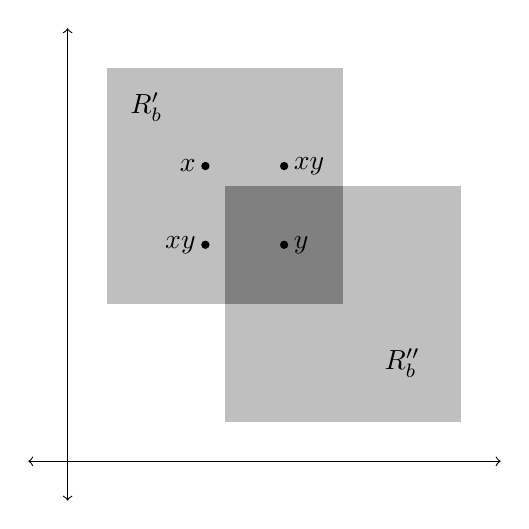
\begin{tikzpicture}[scale=1]
	
	% S'
	\fill[lightgray] (2,0.5)--(5,0.5)--(5,3.5)--(2,3.5);
	\draw (4.25,1.25) node {$R_b''$};

	% S''
	\fill[lightgray] (0.5,2)--(3.5,2)--(3.5,5)--(0.5,5);
	\draw (1,4.5) node {$R_b'$};

	% overlap
	\fill[gray] (2,2)--(3.5,2)--(3.5,3.5)--(2,3.5);

	% points
	\fill (1.75,2.75) circle[radius=1.5pt];
	\fill (2.75,2.75) circle[radius=1.5pt];
	\fill (2.75,3.75) circle[radius=1.5pt];
	\fill (1.75,3.75) circle[radius=1.5pt];

	% point labels
	\draw (1.75,2.75) node[anchor=east] {$x \meet y$};
	\draw (2.75,2.75) node[anchor=west] {$y$};
	\draw (2.75,3.75) node[anchor=west] {$x \join y$};
	\draw (1.75,3.75) node[anchor=east] {$x$};

	% axes
	\draw[<->] (-0.5,0) -- (5.5,0);
	\draw[<->] (0,-0.5) -- (0,5.5);

\end{tikzpicture}